\documentclass[a4paper,12pt,twoside]{article}

\usepackage[left=2.25cm, top=3cm, right=2cm, bottom=3cm]{geometry}
\usepackage{cmap}					          % поиск в PDF
\usepackage[T2A]{fontenc}			      % кодировка
\usepackage[utf8]{inputenc}			    % кодировка исходного текста
\usepackage[english,russian]{babel}	% локализация и переносы
\usepackage{amsmath}	              % локализация и переносы
\setlength{\parindent}{1em}         % отступ в начале каждого параграфа
\usepackage{courier}                % шрифт для кода
\usepackage{mathptmx}               % шрифт Times New Roman
\usepackage{setspace}
\usepackage{relsize}                % большие математические операторы
\usepackage{graphicx}               % картинки
\usepackage{titlesec}
\usepackage{multicol}
\usepackage{color}
\usepackage{caption}                % расстояние от таблицы до названия
\captionsetup[table]{skip=10pt}
%\graphicspath{ {./images/} }
%\полуторный интервал
\onehalfspacing % Интерлиньяж 1.5

\usepackage{fancyhdr} % Колонтитулы

\pagestyle{fancy}
\fancyhf{}
\fancyhead[LE,RO]{2021}
\fancyhead[RE,LO]{Applied econometrics / ПРИКЛАДНАЯ ЭКОНОМЕТРИКА}
\fancyfoot[LE,RO]{\thepage}
\fancyfoot[RE,LO]{Эконометрика}

\renewcommand{\headrulewidth}{2pt}
\renewcommand{\footrulewidth}{1pt}

\title{Анализ волатильности цен акций компаний РФ, осуществляющих торговлю потребительскими товарами}


\begin{document} % Конец преамбулы, начало текста.

\selectlanguage{russian}

\thispagestyle{empty}
\begin{center}
    \textbf{Федеральное государственное автономное образовательное учреждение\\ высшего профессионального образования\\
<<Национальный исследовательский университет\\  <<Высшая школа экономики>>}

    \vspace{8ex}
    \begin{center}
        Факультет экономических наук\\
        \vspace{4ex}
        Образовательная программа <<Финансовые рынки и финансовые институты>>
    \end{center}
\end{center}
\vspace{7ex}

\begin{center}
    {\textbf{ДОМАШНЯЯ РАБОТА ПО ЭКОНОМЕТРИКЕ
    }}
    \vspace{1ex}

    <<Анализ волатильности цен акций компаний РФ, осуществляющих торговлю потребительскими товарами>>
\end{center}
\vspace{20ex}
\begin{flushright}
  \noindent
  Выполнили:\\
  \vspace{1ex}
    \noindent
    Студенты групп № МФР201, МФР202\\
    Апрелев Павел\\
    Волкова Анастасия\\
    Лозовой Владимир


\end{flushright}

\vfill

\begin{center}
    Москва 2021

\end{center}
\newpage


\vspace{25ex}
% Позже здесь будет Аннотация
\begin{center}
  \Large{Анализ волатильности цен акций компаний РФ, осуществляющих торговлю потребительскими товарами}
\end{center}


\definecolor{lgreen}{rgb}{0.9,1,0.8}
\fcolorbox{green}{lgreen}{Позже здесь будет Аннотация}

\titleformat{\section}[block]{\normalfont\Large\centering}{\thesection}{1ex}{}
\section{Построение модели для волатильности цен акций компаний}\label{mgarch}

В данной части будут построены модели волатильности цен акций 4 компаний РФ, осуществляющих торговлю потребительскими товарами (Retail):
MВидео,
Магнит,
Лента,
X5 Retail Group.

Анализируемый промежуток времени: с 01.09.2014 по настоящий момент времени.
Исключением является лишь модель для компании X5 Retail Group, так как для данного эмитента торговля депозитарными расписками на ММВБ началась лишь с 02.02.2018.
Однако данная компания занимает важную нишу на рынке потребительских товаров, поэтому она будет проанализирована на ряду с остальными.

Для всех выбранных компаний был проведен анализ с целью выбора наилучшей спецификации модели.
В данном разделе будет подробно продемонстрирована процедура подбора модели для эмитента M.Video.
Для остальных компаний процедура аналогична.
Результаты будут представлены ниже.

\subsection{Загрузка и обработка данных, сравнительный анализ доходностей}

% Добавить ссылку на парсер
После загрузки данных с Мосбиржи с помощью парсера в Python, проведем в R конвертацию дат в формат дат ('\%Y-\%m-\%d').
Далее будем работать на языке программирования R.

Проведем первичный графический анализ распределений доходностей выбранных эмитентов, а также сравнению их с нормальными. Для этого при помощи команды qplot сравним между собой плотности распределений выбранных компаний – ‘FIVE’, ‘MGNT’, ‘LNTA’, ‘MVID’. Полученные графики представлены ниже [Рис. 1]:

\begin{figure}[!h]
  %\advance\leftskip-1.5cm
    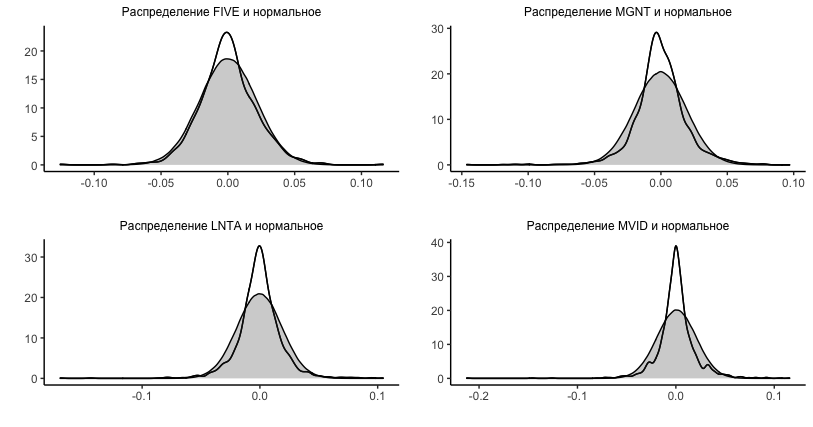
\includegraphics[scale = 0.55]{dist_01.png}
    \caption{Сравнение распределений доходностей эмитентов с нормальным}
    \label{fig:dist_01}
\end{figure}

Полученные распределения доходностей визуально отличаются от нормального.
Тем не менее наиболее приближенно к нему распределение доходностей компании X5 Retail Group, а наименее – распределения доходностей компаний LENTA и M.VIDEO. Коэффициенты эксцесса (меры остроты пика) у этих компаний велики.
Это в свою очередь наталкивает на мысль, что модификации моделей авторегрессии — скользящего среднего (ARMA), а также обобщенной авторегрессионной гетероскедастичности (GARCH) нужно будет строить в соответствие с предпосылкой об отсутствии нормально распределенных ошибок.

\subsection{Построение моделей для компании M.VIDEO}

В наиболее подробном виде нами проведен анализ доходностей и волатильности, а также построение моделей у компании M.VIDEO.

\subsubsection{Проверка на стационарность}

При построении модели для доходностей рассматриваемого эмитента нами будет протестирована модель интегрированной авторегрессии – скользящего среднего (ARIMA).
При выборы спецификации и параметров данной модели мы руководствовались методологией Бокса-Дженкинса (Box, Jenkins).
% Добавить литературу

Первоначально нужно выяснить, является ли ряд стационарным, чтобы понять необходимо ли взятие разностей некоторого порядка исходного временного ряда.
На первый взгляд, исходя из [Рис. 2], полученный ряд напоминает стационарный процесс.
Значения колеблются на одном уровне вокруг нуля.
Устойчивых тенденций не наблюдается.
Перейдем к более детальному исследованию.

\begin{figure}[!h]
  %\advance\leftskip-1.5cm
    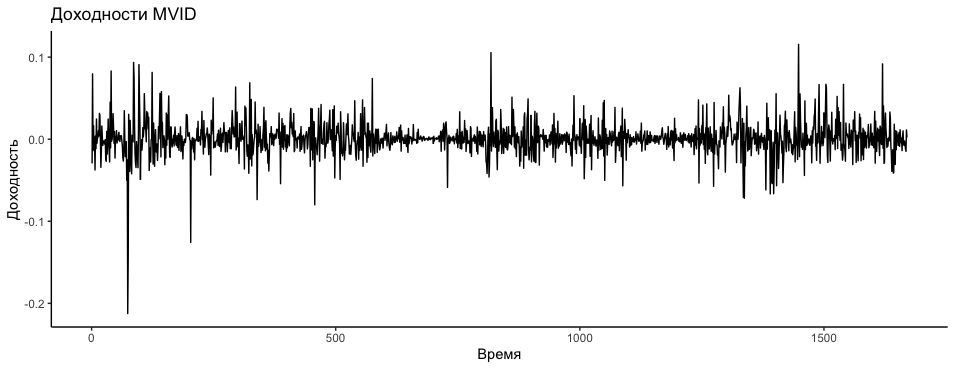
\includegraphics[scale = 0.5]{mvideo_01.png}
    \caption{Доходности MVideo}
    \label{fig:mvideo_01}
\end{figure}

Для формального обоснования необходимо использовать количественную методологию. Наиболее широко распространенной методикой в эконометрике для анализа временных рядов для проверки на стационарность является Расширенный тест Дики – Фуллера (ADF-Тест).

Суть данного теста заключается в проверке нулевой гипотезы о наличии единичного корня.
В данном случае в тестовые регрессии происходит включение лагов первых разностей, так как процесс может быть авторегрессией не первого, а более высокого порядка.
Таким образом, ADF тест применяется к следующей модели:

$$X_t = \mu + \alpha X_{t-1} + \varepsilon_t$$
$$\Delta X_t = X_t-X_{t-1}= \mu + (\alpha-1)X_{t-1} + \varepsilon_t$$
$$\varepsilon_t \sim WN(0, \sigma^2)$$

Модель включает в себя константу и зависимость от предыдущего наблюдения, то есть авторегрессионный процесс.
В уравнении выше представлена авторегрессия первого порядка.
В общем случае проверяется порядок $p$.
Рекомендуется выбрать в качестве значения периода $p$ целую часть от числа $\sqrt[3]{N}$, где $N$ - количество наблюдений, так как эмпирически установлено, что данные компоненты вносят основной вклад.

Проверяется гипотеза о единичном корне.
Она предполагает наличие случайного блуждания.
Альтернатива, что случайного блуждания нет.
$$  H_0: \alpha = 1$$
$$  H_1: \alpha < 1$$
Применяем расширенный критерий Дики-Фуллера (ADF-критерий), статистика которого имеет распределение $DF_{\mu}$.
Если гипотеза о наличии единичного корня отвергается, принимаем вышеуказанную модель и считаем, что процесс стационарен, взятие разностей не необходимо.

В нашем случае для компании MVideo были получены следующая тестовая статистика и уровень значимости:
$$ DF = -26.744$$
$$ p-value = 2.2e-16 $$

Таким образом, нулевая нулевая гипотеза отвергается на любом уровне значимости, что говорит нам об отсутствии единичного корня. А следовательно, можно сделать вывод о том, что процесс является стационарным, а временные ряды подчиняются модели  ARMA (p, q).

\subsubsection{Выбор спецификации модели ARMA}

После того, как мы доказали, что временной ряд доходностей рассматриваемого эмитента является стационарным, перейдем  непосредственно к выбору спецификации модели ARMA.

Изобразим графики автокорреляционной и частичной автокорреляционной функций для идентификации случайной составляющей ряда и выбора подходящих базовых моделей
Во время процедуры идентификации модели следует принимать во внимание оба графика.

\begin{figure}[!h]
  %\advance\leftskip-1.5cm
    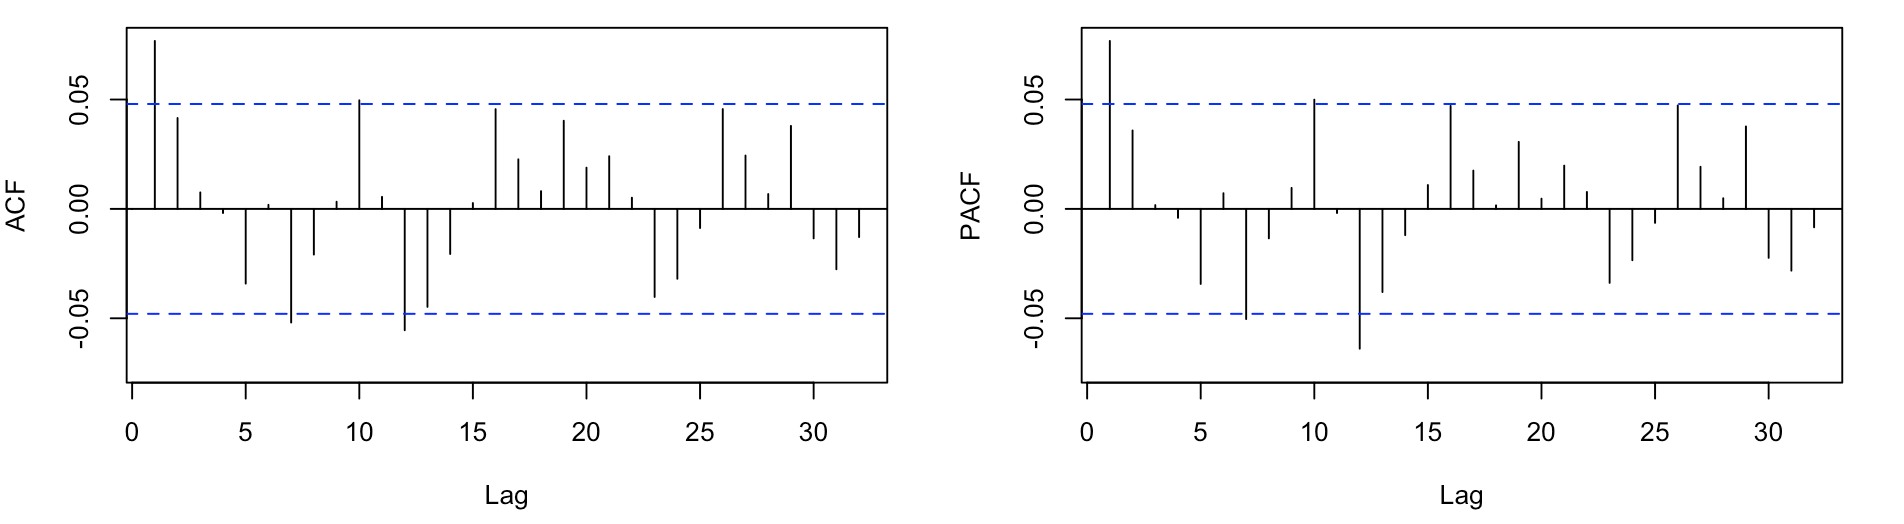
\includegraphics[scale = 0.5]{mvideo_02.png}
    \caption{Доходности MVideo: АКФ, ЧАКФ}
    \label{fig:mvideo_02}
\end{figure}


Для авторегрессионных процессов порядка $p$, первые $p$ лагов ЧАКФ являются значимыми, остальные нулевые (в пределах интервала), а АКФ плавно убывает.
Для MA(q) процессов наоборот.

Для нашего процесса видим, что выборочная АКФ постепенно убывает, заходя на 2 лаге в пределы доверительного интервала (границы соответствуют критическим значениям для 95\% уровня доверия, поделенным на корень из количества наблюдений)
На графике выборочной ЧАКФ наблюдается всплеск первой компоненты, далее значения в пределах доверительноого интервала,кроме небольшого превышения примерно на 12 лаге.
На данном этапе нельзя однозначно сказать к какому типу относится процесс: авторегрессия или скользящее среднее.
Вполне возможна спецификация ARMA, необходимо дальнейшее исследование.

Протестируем несколько моделей.
Формально спецификация модели выбирается в соответствии с значениями информационных критериев - Акаике (AIC) и Шварца (BIC).

$$ AIC = \ln \hat\sigma^2_{\varepsilon} + \frac{2(p+q)}{n}$$
$$ BIC = \ln \hat\sigma^2_{\varepsilon} + (p+q)\frac{\ln(n)}{n}$$

Они показывают меру относительного качества моделей, учитывая степень <<подгонки>> модели под данные с штрафом на используемое количество оцениваемых параметров. Таким образом, их количественные показатели основаны на компромиссе между точностью и сложностью модели.

В результате автоматичекого подбора спецификации модели ARIMA (auto.arima) была выбрана модель ARIMA (3,0,1) со следующими значениями коэффициентов, стандартных отклонений и значений информационных критериев:

\begin{table}[!h]
\centering
\begin{tabular}{lllllll}
  \hline
  & AR1 & AR2 & AR3 & MA1 & AIC & BIC\\
  \hline
  ARIMA(3,0,1) & -0.81 & 0.11 & 0.02 & 0.88 & -8353.42 & -8326.32\\
  \hline
\end{tabular}
\caption{Коэффициенты подобранной модели MVideo}
\end{table}

Тем не менее можно заметить, что коэффициент при AR3 не является значимым на уровне значимости в 5\%, так как если взять разность между коэффициентом и двумя стандартными отклонениями, 0 войдет в доверительный интервал ($0.0201- 2\times0.0275 < 0$). Именно поэтому мы посчитали спецификацию модели ARIMA (2,0,1) наиболее оптимальной.

В заключении проверим визуально наличие условной гетероскедастичности. Для этого изобразим графически квадрат доходностей эмитента M.VIDEO, который является оценкой дисперсии случайной ошибки [Рис. 4]

\begin{figure}[!h]
  %\advance\leftskip-1.5cm
    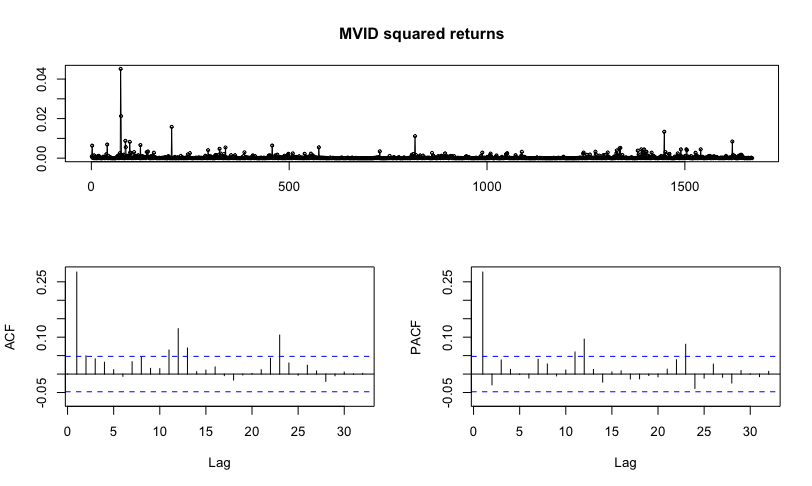
\includegraphics[scale = 0.6]{mvideo_3.png}
    \caption{Доходности MVideo: условная гетероскедастичность}
    \label{fig:mvideo_03}
\end{figure}

Графики автокорреляции (ACF) и частичной автокорреляции (PACF) демонстрируют наличие гетероскедастичности, поэтому необходимо перейти к построению ARIMA-GARCH-модели.

\subsubsection{Выбор спецификации модели GARCH}

Изначально при помощи пакета \textit{rugarch} оценим наиболее адекватную модель, ARIMA (2,0,1) - GARCH(1,1), учитывая, что математическое ожидание ($\mu$) равно нулю.
Таким образом, в соответствии с предыдущей оценкой, уравнение доходности имеет вид:
$$
y_t = \varphi_1 y_{t-1} + \varphi_2 y_{t-2} + \varepsilon_t + \theta_1 \varepsilon_{t-1}
$$

Уравнение волатильности $ \varepsilon_t = \sigma_t z_t $ имеет вид:
$$
\sigma_t^2 = \omega + \alpha_1 \varepsilon_{t-1}^2 + \beta_1 \sigma_{t-1}^2
$$
$$
z_t \sim N \rightarrow \varepsilon_t \sim N
$$

Построим модель ARIMA(2,0,1)-GARCH(1,1) и посмотрим на результаты оценивания:

\begin{table}[!h]
\centering
\begin{tabular}{lllllll}
  \hline
          &  Estimate & Std. Error &  t value  &  Pr(>|t|) \\
  \hline
  ar1 & -0.81 &  0.23 & -3.66 & 0.00 \\
  ar2 & -0.02 &  0.04 & -0.49 & 0.62 \\
  ma1 & 0.72 &  0.21 & 3.29 & 0.00 \\
  $\omega$ & 0.00 &  0.00 & 6.07 & 0.00 \\
  $\alpha_1$ & 0.18 &  0.01 & 10.75 & 0.00 \\
  $\beta_1$ & 0.81 &  0.01 & 81.21 & 0.00 \\
  \hline
\end{tabular}
\caption{Коэффициенты подобранной модели ARIMA(2,0,1)-GARCH(1,1) для MVideo}
\end{table}

Все переменные, кроме ar2, являются значимыми на любом адекватном уровне значимости.
Теперь перейдем непосредственно к проведению тестов для оценки качества модели.

\subsubsection{Тесты полученной ARIMA-GARCH модели}

Теперь нужно провести проверку остатков выбранной модели на белошумность, чтобы проверить адекватность выбранной модели.

Используем критерий Льюнга-Бокса:

$$Q^* = T(T+2) \sum_{k=1}^h (T-k)^{-1}r_k^2$$
$$\text{где } h - \text{максимальный лаг},  T - \text{количество наблюдений}$$

Чем меньше $r_k$, тем меньше итоговая сумма $Q$.
Как правило, рекомендуется брать количество лагов не больше 10, также есть популярный вариант N/5 для небольших выборок.

Критерий предполагает проверку гипотезы о совместном равенстве нулю всех автокорреляций временного (до выбранного момента).
Альтернативная гипотеза предполагает, что остатки не случайны.
Оценивается с помощью выборочной автокорреляции.
Статистика имеет Хи-квадрат распределение.


Данный тест используется для того, чтобы определить, имеет ли место автокорреляции между стандартизированными остатками. Рассматриваются следующие гипотезы:

$$
H_0: \text{no serial correlation}
$$
$$
H_a: \text{serial correlation}
$$

Получаем следующие тестовые статистики и уровни значимости:

\begin{table}[!h]
\centering
\begin{tabular}{lllllll}
  \hline
          &  statistic  &  p-value  \\
  \hline
  Lag[1]  & 4.76 & 0.03 \\
  Lag[2*(p+q)+(p+q)-1][8]  & 6.70 &  0.00 \\
  Lag[4*(p+q)+(p+q)-1][14]  & 8.62 &  0.27 \\
  \hline
\end{tabular}
\caption{Weighted Ljung-Box Test on Standardized Residuals}
\end{table}

Основная гипотеза о белошумности (гауссовости) остатков \textbf{отвергается}, что не подтверждает адекватность выбранной модели.

Таким образом, для всех тестируемых лагов нулевая гипотеза отвергается в пользу альтернативной, а значит остатки в модели коррелированы между собой.
Аналогичные результаты продемонстрированы на [Рис. 5] – для первого лага явно видна значимая автокорреляция:

\begin{figure}[!h]
  %\advance\leftskip-1.5cm
    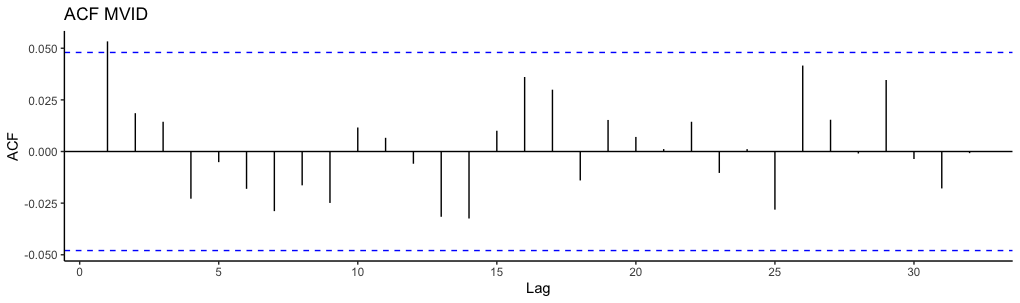
\includegraphics[scale = 0.45]{mvideo_4.png}
    \caption{Автокорреляция стандартизованных остатков}
    \label{fig:mvideo_04}
\end{figure}


Такой же тест проводится для квадратов остатков, полученных из модели.
Если модель достаточно хорошо описывает гетескедастичность, то квадраты остатков не должны быть коррелированы между собой, а представлять собой лишь случайные шоки:

\begin{table}[!h]
\centering
\begin{tabular}{lllllll}
  \hline
          &  statistic  &  p-value  \\
  \hline
  Lag[1]  & 0.02 & 0.88 \\
  Lag[2*(p+q)+(p+q)-1][8]  & 0.62 &  0.94 \\
  Lag[4*(p+q)+(p+q)-1][14]  & 2.18 &  0.88 \\
  \hline
\end{tabular}
\caption{Weighted Ljung-Box Test on Standardized Squared Residuals}
\end{table}

Итак, согласно полученным тестовым статистикам и уровням значимости, для всех лагов нет основания отвергать основную гипотезу, а значит квадраты остатков не связаны между собой – модель волатильности построена корректно. Такие же результаты можно увидеть и графически [Рис. 6] – отсутствует значимая автокорреляция для всех лагов:

\begin{figure}[!h]
  %\advance\leftskip-1.5cm
    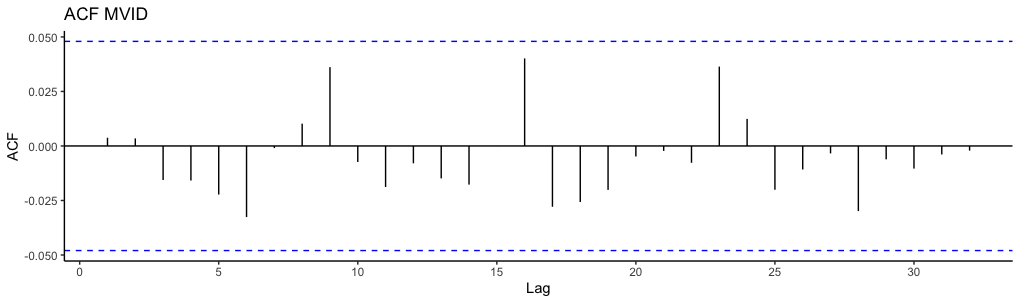
\includegraphics[scale = 0.45]{mvideo_6.png}
    \caption{Автокорреляция квадратов стандартизованных остатков}
    \label{fig:mvideo_06}
\end{figure}

Проведем Sign Bias тест.
Он позволяет узнать, реагирует ли волатильность в различной мере для отрицательных и положительных шоков.  Если получается значимая статистика, то в этом случае имеет смысл построить модель EGARCH. Имеем следующие гипотезы:

$$
H_0: \text{no sign bias}
$$
$$
H_a: \text{sign bias}
$$

Получаем следующие тестовые статистики и уровни значимости:

\begin{table}[!h]
\centering
\begin{tabular}{lllllll}
  \hline
          &  statistic  &  p-value  \\
  \hline
  Sign Bias   & 0.09 & 0.93 \\
  Negative Sign Bias  & 0.12 &  0.91 \\
  Positive Sign Bias  & 0.13 &  0.89 \\
  Joint Effect   & 0.03 &  0.99 \\
  \hline
\end{tabular}
\caption{Sign Bias Test}
\end{table}

Таким образом, во всех случаях мы получаем незначимую тестовую статистику, а значит нет оснований отвергать основную гипотезу об отсутствии асимметрии. Следовательно, необходимости строить модификацию для нашей модели в виде модели EGARCH нет.


\subsubsection{Модификация ARIMA-GARCH модели}

Исходя из полученного графика плотности распределения доходностей компании M.VIDEO [Рис. 1], очевидным становится то, что распределение сильно отличается от нормального.
Следовательно полученную модель необходимо модифицировать с целью получения большего числа наблюдения <<в хвостах>>.
Было решено построить новую модель и ввести предпосылку о том, что остатки распределены в соответствии с распределением Стьюдента:
$$
z_t \sim t \rightarrow \varepsilon_t \sim t
$$

Построим новую модель ARIMA(2,0,1) - GARCH(1,1) и посмотрим на результаты оценивания:


\begin{table}[!h]
\centering
\begin{tabular}{lllllll}
  \hline
          &  Estimate & Std. Error &  t value  &  Pr(>|t|) \\
  \hline
  ar1 & -0.85 &  0.18 & -4.73 & 0.00 \\
  ar2 & -0.03 &  0.03 & -1.09 & 0.28 \\
  ma1 & 0.78 &  0.18 & 4.40 & 0.00 \\
  $\omega$ & 0.00 &  0.00 & 2.36 & 0.02 \\
  $\alpha_1$ & 0.28 &  0.04 & 6.82 & 0.00 \\
  $\beta_1$ & 0.72 &  0.06 & 13.03 & 0.00 \\
  shape & 3.28 &  0.21 & 15.86 & 0.00 \\
  \hline
\end{tabular}
\caption{Коэффициенты подобранной модели ARIMA(2,0,1)-GARCH(1,1) для MVideo}
\end{table}


Как и в предыдущем случае все переменные, кроме ar2, являются значимыми на любом адекватном уровне значимости. Estimate $\sim$ 3.27 у переменной shape, а также p-value $\rightarrow$  0 означают то, что распределение шоков не является нормальным, и оценивание и использованием предпосылки о распределении остатков по Стьюденту действительно имело смысл.
Кроме того, были получены следующие показатели логарфимической функции правдоподобия и информационных критериев:

\begin{table}[!h]
\centering
\begin{tabular}{lllllll}
  \hline
          &  T-distribution & Normal  \\
  \hline
  LogLikelihood & 4605.82 &  4370.58 \\
  Akaike  & -5.51 &  -5.23  \\
  Bayes & -5.48 &  -5.21 \\
  \hline
\end{tabular}
\caption{Сравнение моделей}
\end{table}

Таким образом, при сопоставлении с информационными критериями предыдущей модели можно сделать вывод, что новая модель лучше, так как их величины меньше по абсолютному значению.
Теперь перейдем непосредственно к проведению тестов для оценки качества модели.

Получены следующие показатели:

\begin{table}[!h]
\centering
\begin{tabular}{lllllll}
  \hline
          &  statistic  &  p-value  \\
  \hline
  Lag[1]  & 2.16 & 0.14 \\
  Lag[2*(p+q)+(p+q)-1][8]  & 4.72 &  0.35 \\
  Lag[4*(p+q)+(p+q)-1][14]  & 6.93 &  0.57 \\
  \hline
\end{tabular}
\caption{Weighted Ljung-Box Test on Standardized Residuals}
\end{table}

Можно сделать вывод, что на уровне значимости в 10\% нет основания отвергать основную гипотезу об отсутствии автокорреляции остатков в пользу альтернативной. А значит, модель стала лучше.

Такой же тест проводится для квадратов остатков, полученных из модели.
Если модель достаточно хорошо описывает гетескедастичность, то квадраты остатков не должны быть коррелированы между собой, а представлять собой лишь случайные шоки:

\begin{table}[!h]
\centering
\begin{tabular}{lllllll}
  \hline
          &  statistic  &  p-value  \\
  \hline
  Lag[1]  & 0.39 & 0.54 \\
  Lag[2*(p+q)+(p+q)-1][8]  & 1.38 &  0.77 \\
  Lag[4*(p+q)+(p+q)-1][14]  & 3.04 &  0.75 \\
  \hline
\end{tabular}
\caption{Weighted Ljung-Box Test on Standardized Squared Residuals}
\end{table}

Как и в предыдущем случае, в соответствии в полученными тестовыми статистиками нет оснований отвергать основную гипотезу о наличии автокорреляции между квадратами остатков, модель волатильности построена корректно.

Проведем Sign Bias тест.

Получаем следующие тестовые статистики и уровни значимости:

\begin{table}[!h]
\centering
\begin{tabular}{lllllll}
  \hline
          &  statistic  &  p-value  \\
  \hline
  Sign Bias   & 0.22 & 0.82 \\
  Negative Sign Bias  & 0.99 &  0.32 \\
  Positive Sign Bias  & 0.65 &  0.52 \\
  Joint Effect   & 1.42 &  0.70 \\
  \hline
\end{tabular}
\caption{Sign Bias Test}
\end{table}

Полученные тестовые статистики позволяют сделать вывод об отсутствии основания для отвержения основной гипотезы.
А значит в новой модели отсутствует асимметрия волатильности.

\subsubsection{Сравнение оценок волатильности}

Посмотрим графически, какая из моделей лучше предсказывает всплески волатильности. Для этого на графике построим квадрат доходностей (несмещенная оценка волатильности), а также оценки волатильности, полученные в моделях ARIMA(2,0,1)-GARCH(1,1) с нормальным распределением ошибок и распределением ошибок по Стьюденту [Рис. 7]:

\begin{figure}[!h]
  %\advance\leftskip-1.5cm
    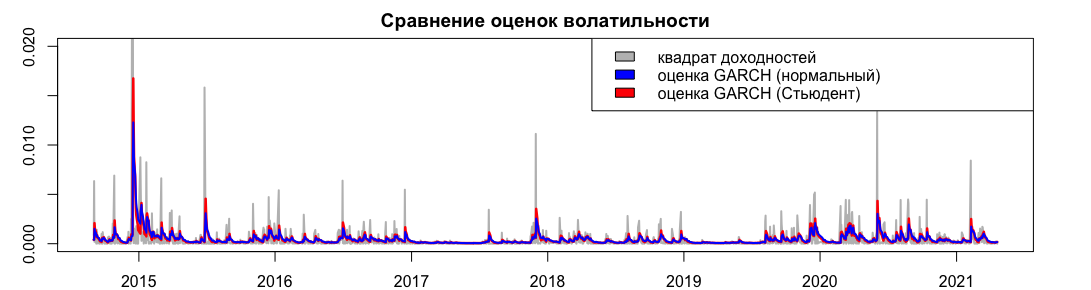
\includegraphics[scale = 0.46]{mvideo_8.png}
    \caption{Сравнение оценок волатильности}
    \label{fig:mvideo_08}
\end{figure}

Можно заметить, что оценка модели GARCH с распределением шоков по Стьюденту лучше предсказывает всплески волатильности, потому что распределение имеет более тяжелые <<хвосты>>.
Таким образом, построенная новая модель, где берется предпосылка о распределении шоков по Стьюденту лучше в соответствии со следующими критериями:
\begin{itemize}
  \item Информационные критерии у новой модели имеют более низкие показатели по абсолютному значению
  \item Weighted Ljung-Box Test on Standardized Residuals показал отсутствие автокорреляции стандартизированных остатков, распределение шоков не является нормальным
  \item Визуально можно убедиться в том, что новая модель лучше предсказывает всплески волатильности [Рис. 7]
\end{itemize}

\subsubsection{Прогноз волатильности}
В соответствии с построенной моделью ARIMA(2,0,1)-GARCH(1,1) построим прогноз волатильности на 10 дней и сравним с полученной оценкой за последний квартал [Рис. 8]:

\begin{figure}[!h]
  %\advance\leftskip-1.5cm
    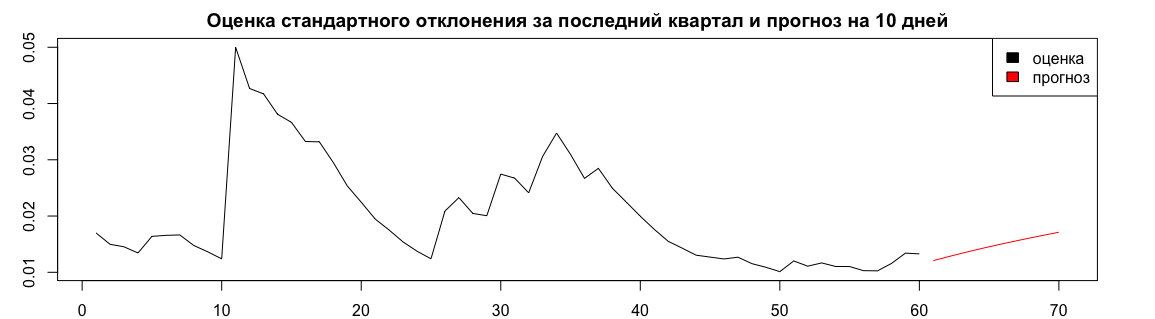
\includegraphics[scale = 0.43]{mvideo_9.png}
    \caption{Сравнение оценок волатильности}
    \label{fig:mvideo_09}
\end{figure}

Таким образом, построенная нами модель четко уловила то, что за первичным ростом волатильности идет еще больший ее рост.

\subsection{Построение моделей доходностей и волатильности остальных эмитентов}

Перейдем к построению моделей уже для остальных эмитентов.
В этом разделе процесс выбора спецификации моделей и проведение тестов будет описано не так подробно, а отражены лишь основные полученные результаты.

\subsubsection{Проверка на стационарность временного ряда остальных компаний}

Начнем анализ временных рядов доходностей остальных эмитентов с проверки всех трех динамик доходностей на стационарность.
Аналогичным образом проведем расширенный тест Дики Фуллера (ADF-test) на наличие единичного корня.
Получим следующие тестовые статистики для эмитентов:

\begin{table}[!h]
\centering
\begin{tabular}{lllllll}
  \hline
          & DF-statistics &  p-value  \\
  \hline
  MGNT   & -28.59 & 2.2e-16 \\
  LNTA  & -29.16 &  2.2e-16 \\
  X5 RETAIL  & -19.79 &  2.2e-16 \\
  \hline
\end{tabular}
\caption{Результат ADF-теста для проверки стационарности}
\end{table}

Таким образом, для всех трех эмитентов, MGNT, LNTA, X5 RETAIL, временные ряды доходностей являются стационарными, а значит не нужно брать разность какого-либо порядка при построении ARIMA-модели.

\subsubsection{Выбор спецификации для моделей ARIMA}

Для всех трех выбранных временных рядов происходит выбор спецификации моделей ARIMA при помощи команды auto.arima на основе получаемых при разных вариациях значениях информационных критериев Акаике (AIC).
Во всех трёх случаях была выбрана модель ARIMA(0,0,0), а значит фактически можно сделать вывод о том, что доходности представляют собой белый шум. Расчетные показатели совпадают и с графическими наблюдениями – во всех случаях на графиках автокорреляций (ACF) и частичных автокорреляций (PACF) нет значимых показателей.
При визуальном анализе динамики квадратов доходностей у всех трёх эмитентов наблюдается выраженная условная гетероскедастичность, так как заметна значимая автокорреляция на графиках ACF и PACF. Иллюстрации продемонстрированы в приложениях.

\subsubsection{Выбор спецификации для моделей GARCH}

Как и ранее, при помощи пакета rugarch оценим для всех трёх эмитентов ARIMA (0, 0, 0)-GARCH(1, 1) модели, учитывая, что математическое ожидание ($\mu$) равно нулю.
Были получены следующие результаты:

\begin{table}[!h]
\centering
\begin{tabular}{lllllll}
  \hline
          &  MGNT & LNTA &  FIVE \\
  \hline
  $\omega$ & 0.000022 &  0.000028 & 0.000029  \\
  $\alpha_1$ & 0.076808 &  0.225087 & 0.082198 \\
  $\beta_1$ & 0.862237 &  0.713065 & 0.849962 \\

  \hline
\end{tabular}
\caption{Оценки модели ARIMA(0,0,0)-GARCH(1,1) для всех эмитентов}
\end{table}

Кроме того, как и в предыдущем случае, мы провели ряд тестов для выбранных моделей. Weighted Ljung-Box Test on Standardized Residuals показал, что для уровня значимости в 5\% частично отвергается (для некоторых лагов) гипотеза об отсутствии автокорреляции между стандартизированными остатками для MGNT и LNTA. Кроме того, по результатам Weighted Ljung-Box Test on Standardized Squared Residuals можно сделать вывод о том, что на уровне значимости в 5\% нет оснований отвергать основную гипотезу об отсутствии автокорреляции между квадратами остатков всех эмитентов, а значит модель волатильности построена корректно.
Тем не менее, Sign Bias Test показал значимую тестовую t-статистику для компании MGNT: 2.4427 для Negative Sign Bias и 6.6295 для Join Effect, соответственно.
Именно поэтому в дальнейшем проведем для данного эмитента модификацию данной модели в рамках экспоненциальной модели EGARCH.

\subsubsection{Модификация ARIMA-GARCH моделей для MGNT, LNTA, X5 RETAIL}

Исходя из функции распределения плотностей [Рис. 1] всех трех эмитентов, можно также заметить, что распределение доходностей далеко от нормального.
Таким образом, учтем асимметрию для эмитента MGNT (путем построения экспоненциальной модели EGARCH) и островершинность распределения всех трех рядов путем введения предпосылки о распределении шоков по Стьюденту.
Получим следующие результаты:

\begin{table}[!h]
\centering
\begin{tabular}{lllllll}
  \hline
          & eGarch(1,1) MGNT & Garch(1,1) LNTA &  Garch(1,1) FIVE \\
  \hline
  $\omega$ & -0.395060*** &  0.000025*** & 0.000020*  \\
  $\alpha_1$ & -0.051318*** &  0.256280*** & 0.065178*** \\
  $\beta_1$ & 0.950538*** &  0.710732*** & 0.888875*** \\
  $\gamma_1$ & 0.183925*** &  - & - \\
  $shape$ & 4.173907*** &  4.260734*** & 8.350188*** \\
  \hline
\end{tabular}
\caption{Оценки модели ARIMA(0,0,0)-GARCH(1,1) для всех эмитентов}
\end{table}


Полученные результаты позволяют сделать вывод о значимости коэффициентов модели для всех трех эмитентов. Кроме того, коэффициенты при переменной shape говорят нам о том, что распределения случайных ошибок действительно не являются нормальными, наименее выраженный результат у бумаги FIVE.

Для модифицированных моделей были также проведены тесты. Weighted Ljung-Box Test on Standardized Residuals по-прежнему показывает, что для уровня значимости в 5\% частично отвергается (для некоторых лагов) гипотеза об отсутствии автокорреляции между стандартизированными остатками для MGNT и LNTA. В модифицированных моделях по результатам Weighted Ljung-Box Test on Standardized Squared Residuals также можно сделать вывод о том, что на уровне значимости в 5\% нет оснований отвергать основную гипотезу об отсутствии автокорреляции между квадратами остатков всех эмитентов, а значит модель волатильности построена корректно. Построение модели ARIMA(0, 0, 0)-eGarch(1, 1) для компании MGNT нивелировало проблему асимметрии волатильности – все тестовые статистики Sign Bias Test оказались незначимыми на 5\% уровне значимости.

\subsubsection{Сравнение моделей волатильности для MGNT, LNTA, X5 RETAIL}

Проведенные графические и тестовые сравнения позволили выделить преимущества модифицированных моделей волатильности для всех трёх эмитентов, в которых учитывается асимметрия и островершинность распределения.
Тем не менее, проведем более формализованное сравнение этих моделей на основании информационных критериев Акаике (AIC) и Шварца (BIC):

\begin{table}[!h]
\centering
\begin{tabular}{llrrrr}
  \hline
          & & Garch(1,1) & GARCH/eGARCH (1, 1) with t-errors \\
  \hline
  MGNT & AIC &  -5.15 & -5.26  \\
       & BIC &  -5.14 & -5.25 \\
  \hline
  LNTA & AIC &  -5.34 & -5.45 \\
       & BIC &  -5.33 & -5.44 \\
  \hline
  X5 RETAIL & AIC &  -4.94 & -4.96 \\
            & BIC &  -4.92 & -4.93 \\
  \hline
\end{tabular}
\caption{Сравнение моделей волатильности}
\end{table}

Таким образом, мы можем сделать вывод, что полученные модифицированные модели имеют меньшие по абсолютному значению показатели информационных критериев, следовательно, обладают лучшей описательной и прогнозной силой.

\subsection{Сравнение волатильности компаний}

Для каждой бумаги была подобрана и оценена модель волатильности.
Cравним рассматриваемые бумаги по данным показателям.

\begin{table}[!h]
\centering
\begin{tabular}{lrrrr}
  \hline
    SE      & mean & median & lowest & highest \\
  \hline
  MGNT & 0.0191 &  0.018 & 0.010 & 0.054\\
  MVID & 0.0187 &  0.016 & 0.008 & 0.036\\
  LNTA & 0.0183 &  0.016 & 0.009 & 0.099\\
  X5 RETAIL & 0.0210 &  0.019 & 0.015 & 0.049 \\
  \hline
\end{tabular}
\caption{Анализ волатильности}
\end{table}

Наиболее волатильны депозитарные расписки группы X5.
Далее следуют акции Магнита, за ними Мвидео и Лента.
Однако для Ленты наблюдаются более сильные колебания.
Далее перейдем к расчету Value at Risk.
\fcolorbox{green}{lgreen}{Комментарии по смыслу}

\newpage
\section{Value at Risk}

Основываясь на построенных одномерных моделях волатильности, для каждой бумаги был рассчитан однодневный VaR (Value at Risk — сумма под риском для вероятностей 1\% и 5\%)


\begin{figure}[!h]
  %\advance\leftskip-1.5cm
    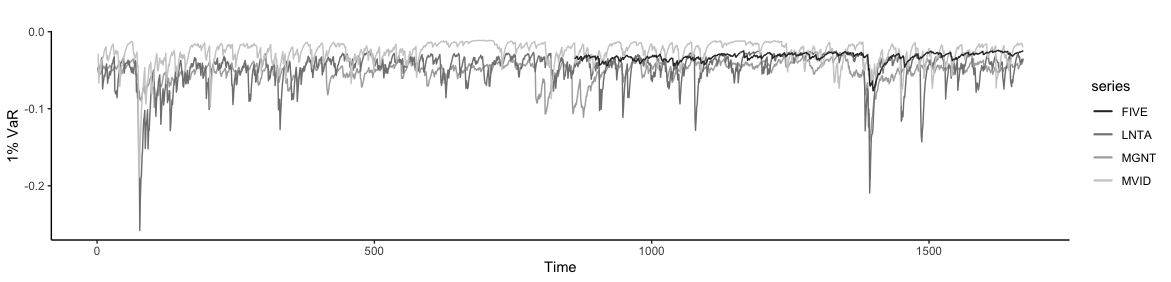
\includegraphics[scale = 0.4]{var_1p.png}
    \caption{Value at Risk 1\%}
    \label{var_1p}
\end{figure}

С точки зрения VaR, более рисковой бумагой является X5 Retail.
За ним следует Лента и Магнит.
Более стабильны акции Мвидео.

\begin{figure}[!h]
  %\advance\leftskip-1.5cm
    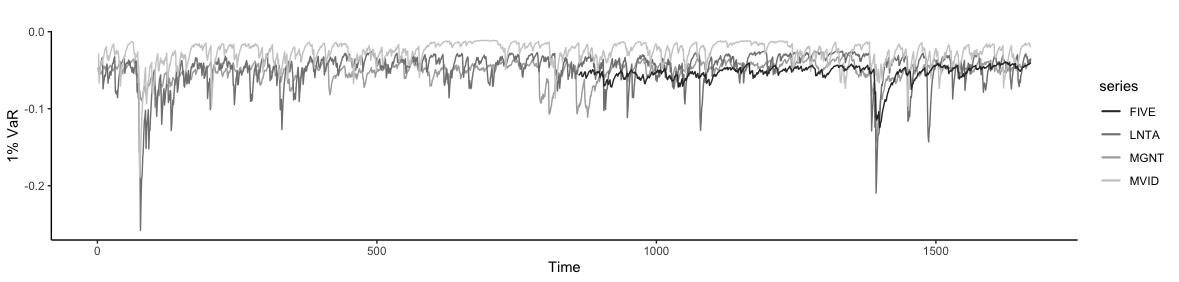
\includegraphics[scale = 0.4]{var_5p.png}
    \caption{Value at Risk 5\%}
    \label{var_5p}
\end{figure}




Также для каждой бумаги был рассчитан VaR на один день вперёд.

\begin{table}[!h]
\centering
\begin{tabular}{lrrrr}
  \hline
          & 1\% VaR & 5\% VaR \\
  \hline
  MGNT & -0.035 &  -0.019 \\
  MVID & -0.017 &  -0.007 \\
  LNTA & -0.036 &  -0.018 \\
  X5 RETAIL & -0.039 &  -0.024 \\
  \hline
\end{tabular}
\caption{Прогноз VaR на 1 шаг вперед}
\end{table}

\fcolorbox{green}{lgreen}{Комментарии по смыслу}






\newpage
\section{Многомерные модели. Формулировка DCC-GARCH модели}\label{mgarch}

\subsection{Выбор модели}\label{model selection}
% R. F. Engle, Dynamic conditional correlation - a simple class of multivariate  garch models. UCSD, May 2001.

Существует несколько наиболее распространённых спецификаций моделей многомерной волатильности, особенности которых достаточно хорошо изучены в научной литературе: VECH, BEKK, DCC-GARCH. С учётом ограниченного размера набора данных, рассматриваемого в данной работе (810 торговых дней, когда известны котировки для всех четырёх акций), и необходимости проведения бэктеста для значений Value at Risk, рассчитанных по многомерной модели, нами было принято решение выбрать спецификацию для многомерной модели, которая бы потребовала оценки минимального числа параметров. Для четырёх активов без учёта модели среднего:
\begin{itemize}
    \item VECH требует оценить 210 параметров.
    \item BEKK требует оценить 42 параметра.
    \item DCC-GARCH необходимо оценить 15 параметров.
\end{itemize}

Исходя из сравнения, нами была выбрана DCC-GARCH модель. DCC-GARCH (Dinamic Conditional Correlation - GARCH) была предложена (Engle, 2001). В общем виде она может быть описана следующим образом:
\begin{equation}
\begin{aligned}
               r_t = \mu_t + \varepsilon_t \\
               \varepsilon_t = H^{1/2}_t z_t
\end{aligned}
\end{equation}

Где:
\begin{itemize}
    \item $r_t$ : $n \times 1$ вектор логарифмических доходнотсей $n$ активов в момент времени $t$.
    \item $\varepsilon_t$: $n \times 1$ вектор стандартизованных доходностей $n$ активов в момент времени $t$, т. е.
          \begin{enumerate}
                \item $E[\varepsilon_t]=0$
                \item $Var[\varepsilon_t] = Ht$
          \end{enumerate}
    \item $\mu_t$: $n \times 1$ вектор математических ожиданий условных доходностей $r_t$ (порождается моделью среднего для доходности).
    \item $H_t$: $n \times n$ матрица условной дисперсии в момент $t$.
    \item $H^{1/2}_t$ : Любая матрица размерности $n \times n$ в момент времени $t$, такая что $H_t$ - матрица условной дисперсии $\varepsilon_t$. $H^{1/2}_t$ может быть получена путем разложения Холецкого $H_t$.
    \item $z_t$: $n \times 1$ вектор независимых и одинаково распределённых случайных величин, таких что $E[z_t]=0$ и $E[z^{T}_t z_t] = I$.
\end{itemize}

Для модели DCC-GARCH изучены и реализованы следующие распределения случайной ошибки $\varepsilon_t$:

\begin{enumerate}
    \item $\varepsilon_t \sim \mathrm{Normal}$.
    \item $\varepsilon_t \sim \mathrm{Student}$.
    \item $\varepsilon_t \sim \mathrm{Laplace}$.
\end{enumerate}

Модель среднего $\mu$ может быть выбрана ислледователем в зависимости от предполагаемых особенностей временного ряда; так, в статистических пакетах языка \texttt{R} реализована возможность оценки AR, MA, ARIMA, ARFIMA, а также константной модели среднего для DCC-GARCH.

Ключевой элемент DCC-GARCH - спецификация модели для $H_t$. Ковариационная матрица раскладывается на произведение матриц стандартных отклонений и корреляционной матрицы:
$$
H_t = D_t R_t D_t
$$
Ковариационная матрица $D_t$ диагональна, $d_{ii}$ представляют собой оценки стандартного отклонения, полученные с помощью одномерных GARCH(p, q) моделей для каждого актива в отдельности:
$$
\begin{gathered}
D_t = \begin{pmatrix}
    \sqrt{h_{1t}} & 0 & \dots \\
    \vdots & \ddots & \\
    0 &  & \sqrt{h_{nt}}
    \end{pmatrix}       \\[2ex]
%\setlength{\jot}{3}
h^{2}_{ii}= \omega +
            \mathlarger{\mathlarger{\sum}}_{q=1}^{Q_i} \alpha_{qi} \varepsilon^{2}_{t-j} +
            \mathlarger{\mathlarger{\sum}}_{p=1}^{P_i} \beta_{pi} h^{2}_{t-i}
\end{gathered}
$$

Корреляционная матрица $R$ оценивается для стандартизированных случайных шоков $\xi_t = D^{-1}_t \varepsilon_t \sim \mathrm{N}(0, R_t)$.Она положительно определена, $\rho_{ii}=1, i=1, ..., n$, и описывается уравнениями:
$$
\begin{gathered}
R_t = Q^{*-1}_t Q_t Q^{*-1}_t \\[2ex]
Q_t = (1-a-b) \overline{Q} + a \xi_{t-1} \xi^{T}_{t-1} + b Q_{t-1} \\[2ex]
\overline{Q} = \frac{1}{T} \mathlarger{\mathlarger{\sum}}_{t=1}^{T} \xi_t \xi^{T}_t
\end{gathered}
$$

Где $a$, $b$ - скаляры, матрица $\overline{Q}$, как следует из уравнений выше - просто оценка средней корреляции, $Q^{*-1}_t$ - матрица нормировки, которая приводит итоговые значения на диагонали оценённой корреляционной матрицы к единице.

\subsection{Выбор спецификации одномерных моделей}\label{specification}

Модель DCC-GARCH обладает одной привлекательной для исследователя особенностью - она позволяет оценить динамические корреляции между отдельными переменными и спрогнозировать их динамику. Это особенно актуально для рассматриваемых компаний X5 Retail Group (далее FIVE), Магнит (MGNT), Лента (LNTA), М.Видео (MVID). Первые три из перечисленных занимают три первых места по выручке среди розничных продуктовых сетей в России, и потому мы ожидаем высокую корреляцию между ними, существенно изменяющуюся во времени в силу фундаментальных показателей эмитентов. Что касается М.Видео, то этот эмитент, по нашим предположениям до оценивания модели, был наименее коррелирован с остальными и поэтому был включён в гипотетический портфель с целью диверсификации рисков.

До оценивания модели рассмотрим выборочные характеристики многомерного набора данных. Мы можем построить скользящие корреляции, чтобы проверить осмысленность выбора спецификации многомерной модели и наличие значимой и высокой корреляции между эмитентами. Отдельно рассмотрим выборочные корреляции MVID с остальными активами.

\begin{figure}[h]
  %\advance\leftskip-1.4cm
    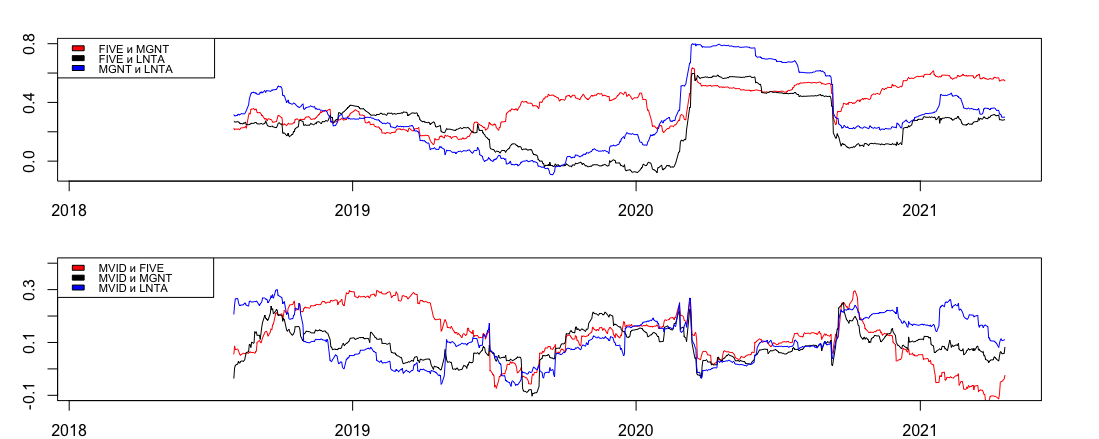
\includegraphics[scale = 0.45]{mult_corr_1.png}
    \caption{Выборочные корреляции}
    \label{fig:rollcorr1}
\end{figure}

Как видно из Рис. \ref{fig:rollcorr1}, М.Видео действительно демонстрирует более низкую корреляцию с другими активами, чем те между собой. Интересно, что корреляция LNTA с FIVE и MGNT значительно снизилась в 2019 году. Это объясняется тем, что Лента показывала слабую операционную и финансовую динамику: гипермаркеты, составляющие существенную часть магазинов сети, потеряли свою привлекательность для потребителя. Более того, летом 2019 года Лента впервые отчиталась о квартальном убытке, что не могло не повлиять на отношение инвесторов к эмитенту. Ситуация изменилась с началом пандемии, когда все сети испытали рост среднего чека в связи с паникой населения, и корреляции между тройкой лидеров продуктового ритейла существенно выросли.

Перейдем непосредственно к построению многомерной модели DCC-GARCH. Поскольку на диагоналях матрицы стандартных отклонений $D_t$ стоят оценки волатильности, полученные из одномерных GARCH-моделей, необходимо выбрать спецификацию модели среднего и волатильности для каждой из них. Эти спецификации могут существенно отличаться от тех, которые были выбраны при оценке одномерных моделей в первой части работы, поскольку торги акциями X5 Retail Group начались только в 2018 году, что укорачивает исходный набор данных наполовину.

Для предварительной диагностики при выборе модели среднего рассмотрим выборочные ACF И PACF каждого ряда.

\begin{figure}[h]
  %\advance\leftskip-1.5cm
    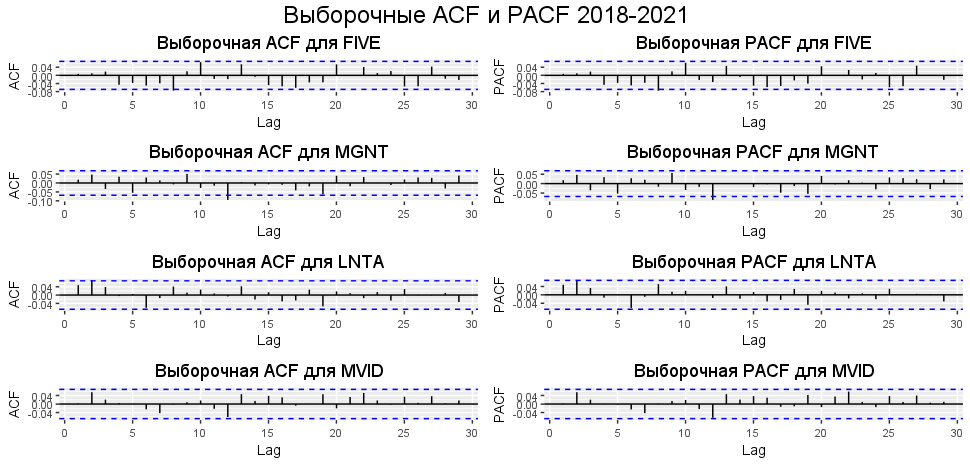
\includegraphics[scale = 0.45]{dcc_acf_pacf.png}
    \caption{Выборочные ACF и PACF}
    \label{fig:acfpacf}
\end{figure}

Рис. \ref{fig:acfpacf} явственно демонстрирует отсутствие значимых лагов, а также сигнализирует о стационарности рядов (тест Дики-Фуллера был проведён при оценке одномерных моделей и показал стационарность всех четырёх рядов). Таким образом, моделью среднего для всех четырёх рядов будет выступать ARIMA(0,0,0).

Визуальная диагностика коррелограмм квадратов доходностей (являющихся несмещённой оценкой дисперсии рядов) свидетельствует о наличии выраженной условной гетероскедастичности, как и при оценке одномерных моделей. С целью уменьшить параметризацию оцениваемой модели и повысить робастность оценок, мы решили использовать стандартную GARCH(1,1) в качестве модели волатильности для всех активов.

\subsection{Результаты оценивания}\label{estimation}
При оценке DCC-GARCH модели были получены следующие оценки коэффициентов:
% Table generated by Excel2LaTeX from sheet 'DCC-GARCH coef'
\begin{table}[htbp]
  \centering
  \captionsetup{font=large}
  \caption{Оценки коэффициентов DCC-GARCH}

    \begin{tabular}{lcccc}
        &  Estimate &  Std. Error &  t value & Pr(>|t|) \\
    FIVE.$\omega$ & 0.000 & 0.000 & 2.138 & 0.033 \\
    FIVE.$\alpha_1$ & 0.082 & 0.028 & 2.943 & 0.003 \\
    FIVE.$\beta_1$ & 0.850 & 0.046 & 18.432 & 0.000 \\
    $\mathbf{MGNT.\omega}$ & $\mathbf{0.000}$ & $\mathbf{0.000}$ & $\mathbf{0.841}$ & $\mathbf{0.401}$ \\
    MGNT.$\alpha_1$ & 0.088 & 0.021 & 4.107 & 0.000 \\
    MGNT.$\beta_1$ & 0.858 & 0.092 & 9.306 & 0.000 \\
    $\mathbf{LNTA.\omega}$ & $\mathbf{0.000}$ & $\mathbf{0.000}$ & $\mathbf{1.016}$ & $\mathbf{0.309}$ \\
    LNTA.$\alpha_1$ & 0.302 & 0.101 & 3.000 & 0.003 \\
    LNTA.$\beta_1$ & 0.639 & 0.159 & 4.017 & 0.000 \\
    $\mathbf{MVID.\omega}$ & $\mathbf{0.000}$ & $\mathbf{0.000}$ & $\mathbf{0.757}$ & $\mathbf{0.449}$ \\
    MVID.$\alpha_1$ & 0.264 & 0.126 & 2.096 & 0.036 \\
    MVID.$\beta_1$ & 0.687 & 0.210 & 3.273 & 0.001 \\
    $\mathbf{DCC.a_1}$ & $\mathbf{0.023}$ & $\mathbf{0.012}$ & $\mathbf{1.955}$ & $\mathbf{0.051}$ \\
    $\mathbf{DCC.b_1}$ & $\mathbf{0.897}$ & $\mathbf{0.073}$ & $\mathbf{12.324}$ & $\mathbf{0.000}$ \\
    $\mathbf{JointStShape}$ & $\mathbf{5.963}$ & $\mathbf{0.430}$ & $\mathbf{13.881}$ & $\mathbf{0.000}$ \\
    \end{tabular}%
  \label{tab:addlabel}%
\end{table}%

Обращают на себя внимание три факта:
\begin{enumerate}
    \item Для всех компаний, кроме X5 Retail Group, коэффициент $\omega$ в одномерных моделях волатильности незначим. Но поскольку изначально мы предполагали, что существует средняя волатильность для каждого эмитента, было бы неразумно подбирать коэффициенты по результатам оценивания модели.
    \item P-value коэффициента DCC.$a_1$, который для уравнения корреляционной матрицы $Q_t$ показывает зависимость текущего значения матрицы от корреляции случайных шоков один период назад, составляет 0.051. В то же время, коэффициент DCC.$b_1$, который отвечает за связь текущего значения корреляционной матрицы со своим предыдущим значением, значим на любом уровне доверия, что позволяет подтвердить препосылку о динамическом характере корреляционной матрицы.
    \item Число степеней свободы многомерного распределения Стьюдента JointStShape равно 5.96, и этот параметр также значим на любом уровне доверия. Сравнительно небольшое число степеней свободы, при котором распределение Стьюдента совсем не похоже на нормальное, подтверждает верность выбора робастного распределения случайных ошибок.
\end{enumerate}

Тест Льюнга-Бокса, проведённый для стандартизованных остатков модели, показал отсутствие автокорреляции для всех рядов на любом уровне значимости, что подтверждает корректность спецификации моделей среднего. Также тест показал отсутствие автокорреляции квадратов остатков, что указывает на адекватный выбор одномерных моделей условной дисперсии.

С целью статистической проверки того факта, что корреляционная матрица меняется во времени (а значит, построение модели DCC-GARCH имело смысл), нами был проведён тест на неизменную корреляцию, впервые предложенный в работе ... . P-value теста составило $0.034$, что на $5\%$ уровне значимости позволяет отвергнуть нулевую гипотезу о константной корреляционной матрице.

Поскольку М.Видео показывает в среднем более низкие значения корреляции с другими эмитентами, чем те между собой, что объясняется низкой ликвидностью акций М.Видео и принадлежностью компании к другому сегменту отрасли (тоже розничная торговля, но электроникой, а не продуктами, как остальные эмитенты в выборке), нами также был рассмотрен вариант построения модели DCC-GARCH для трёх эмитентов без М.Видео. Если выборочные корреляции Пирсона М.Видео с остальными эмитентами оказались бы незначимы на уровне $5\%$, нами была бы оценена новая версия многомерной модели.

% Table generated by Excel2LaTeX from sheet 'corr matrix p-values'
\begin{table}[htbp]
  \centering
  %\captionsetup{font=large}
  %\caption{P-values выборочной \\ корреляционной матрицы}
    \begin{tabular}{lcccc}
      \hline
          & FIVE  & MGNT  & LNTA  & MVID \\
      \hline
    FIVE  & -     & 0.000 & 0.000 & 0.003 \\
    MGNT  & 0.000 & -     & 0.000 & 0.052 \\
    LNTA  & 0.000 & 0.000 & -     & 0.001 \\
    $\mathbf{MVID}$ & $\mathbf{0.003}$ & $\mathbf{0.052}$ & $\mathbf{0.001}$ & $\mathbf{-}$ \\
    \hline
    \end{tabular}%
  \label{tab:addlabel}%
\end{table}%

Но p-значения корреляционной матрицы свидетельствуют о том, что корреляции М.Видео значимы. Поэтому мы решили оставить исходную спецификацию модели и использовать её для прогнозирования, расчёта Value at Risk и проведения бэктеста.

\subsection{Прогнозирование}\label{forecasting}

Как уже было сказано выше, привлекательная особенность модели DCC-GARCH - возможность получить ежедневные оценки и прогнозы корреляции между отдельными эмитентами.

В качестве примера рассмотрим оценки корреляции Xr Retail Group с Магнитом и сравним их с различными выборочными расчётами.

\begin{center}
  \begin{figure}[h]
    %\advance\leftskip-1.2cm
      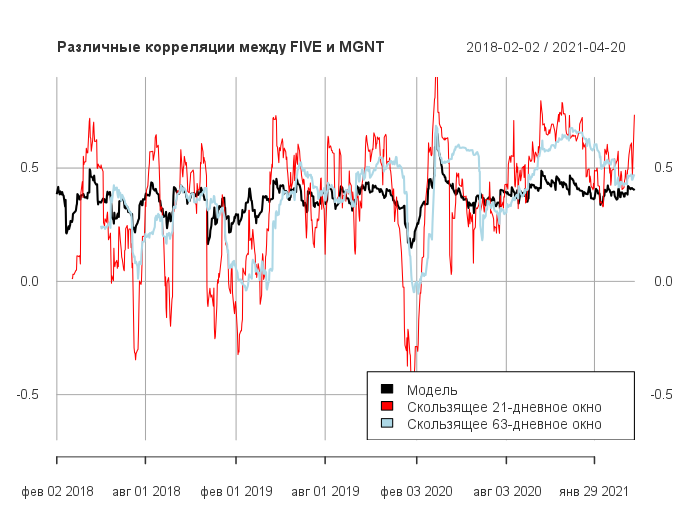
\includegraphics[scale = 0.5]{dcc_five_corrs.png}
      \caption{Различные оценки корреляции X5 Retail Group и Магнита}
      \label{fig:five_mgnt_corrs}
  \end{figure}
\end{center}

Как видно из Рис. \ref{fig:five_mgnt_corrs}, ежедневные оценки корреляции, полученные из модели, представляют собой сглаженный и в то же время более гибкий вариант оценки корреляции: например, шок корреляции, который модель выявила в апреле-марте 2020 года, скользящая полугодовая корреляция учла с заметными запозданием. В то же время, полученные оценки гораздо более стабильны, чем скользящие квартальные корреляции (красная линия).

Заслуживают внимания также краткосрочные прогнозы корреляции, представленные на Рис. %\ref{fig:corr_fcsts}.
М.Видео не изображена на графике как наименее коррелированная с остальными.

%\begin{figure}[h]
%  \advance\leftskip-3.5cm
%    %\centering
%    \includegraphics[width=20cm, height=\textwidth]{corr_forecasts.png}
%    \caption{Оценка и прогноз корреляций}
%    \label{fig:corr_fcsts}
%\end{figure}

Заметно, что модель достаточно точно оценивает краткосрочные тренды корреляции и воспроизводит их в прогнозе.

\subsection{Расчёт VaR и проведение бэктеста}\label{backtesting}
С целью проверки адекватности многомерной модели волатильности нами был проведён её бэктест.
Был сформирован гипотетический портфель, который в равных долях состоит из четырёх акций нашей выборки.
Для этого портфеля на основании предыдущих 126 наблюдений (половина календарного года) оценивалась модель DCC-GARCH в той спецификации, в какой она была оценена выше на всей выборке.
Далее по модели рассчитывался прогноз волатильности и Value at Risk на один период вперёд, прогноз сохранялся.
После этого окно из 126 дней, на котором оценивалась модель, сдвигалось на один период вперёд.
Модель заново оценивалась на новом окне, снова рассчитывались прогнозы.

Таким образом, мы могли оценивать модели скользящим окном начиная со 127 наблюдения.
Поскольку в выборке было 810 торговых дней, мы получили $810-127=683$ прогноза условной волатильности, на основе которых рассчитали Value at Risk.

Каждое наблюдение с отрицательной доходностью, для которого прогнозный VaR по модулю оказался меньше, чем модуль фактической доходности, мы будем далее называть <<пробоем>>.
<<Пробой>> возникает, когда модель недооценила риск портфеля.
Для $5\%$ VaR мы ожидали получить приблизительно $683\times0.05=34$ пробоев, для $1\%$ VaR $683\times0.01=7$.

По результатам бэктеста было получено 9 пробоев для $1\%$ VaR и 33 пробоя для $5\%$ (см. Рис. \ref{fig:backtest}).
Чтобы оценить со статистической точки зрения результат, мы провели тест Купика, нулевая гипотеза которого предполагает равенство ожидаемого числа пробоев наблюдаемому. P-value для $1\%$ VaR составило $42\%$, для $5\%$ VaR - $82\%$. Таким образом, тест Купика подтвердил корректность использования модели для оценки риска портфеля.

  \begin{figure}[h]
   %\advance\leftskip-1.5cm
      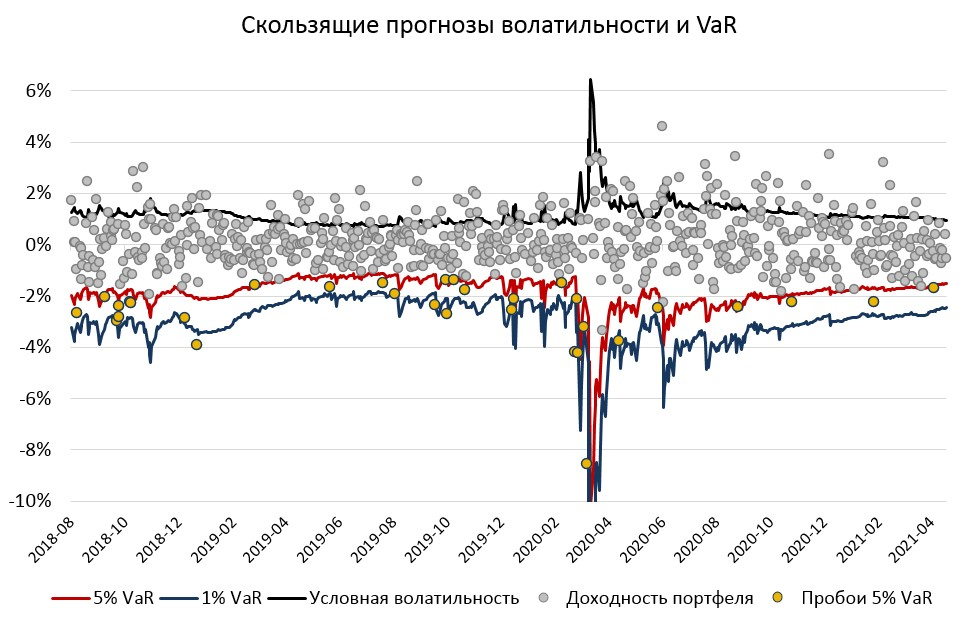
\includegraphics[scale = 0.7]{backtest.jpg}
      \caption{Бэктест DCC-GARCH модели: скользящее 126-дневное окно, \\ прогноз на 1 период вперёд }
      \label{fig:backtest}
  \end{figure}


Также мы рассчитали Value at Risk на один день вперёд. На уровне $1\%$ он составил $1.40\%$ стоимости портфеля, на уровне $5\%$ - $2.27\%$ стоимости портфеля. По сравнению с Value at Risk для одномерных активов, ДОБАВИТЬ РЕЗУЛЬТАТЫ ДЛЯ ОДНОМЕРНЫХ. Стоит отметить, что сравнение приводится для прогноза на конкретную дату (на 21 апреля 2021 года).

\newpage
\section{Приложение}
\begin{figure}[!h]
  \begin{multicols}{2}
    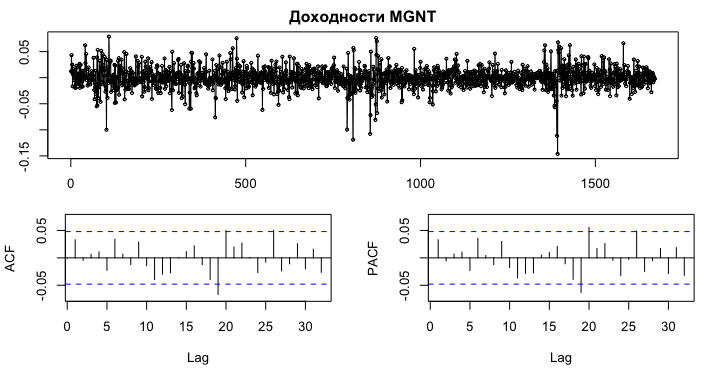
\includegraphics[width=80mm]{magnit_1.png} \hfill
    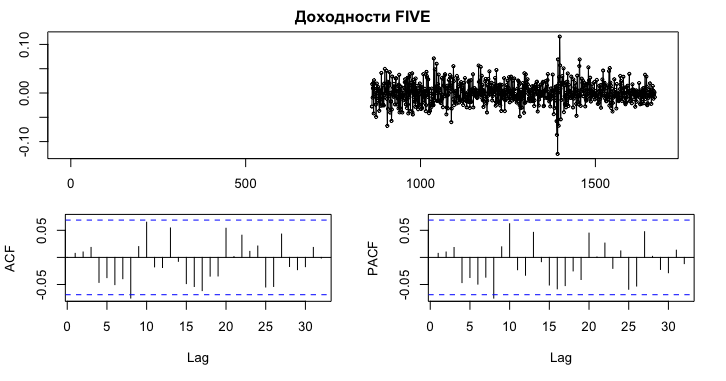
\includegraphics[width=80mm]{five_1.png} \hfill
    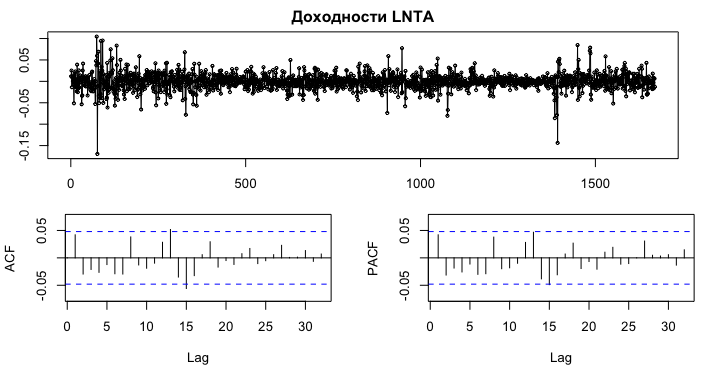
\includegraphics[width=80mm]{lenta_1.png} \hfill
    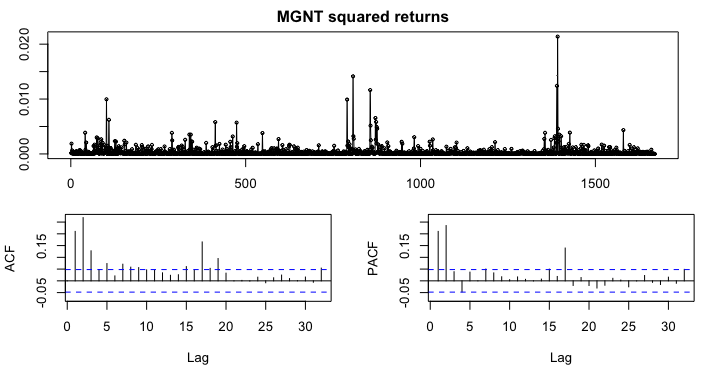
\includegraphics[width=80mm]{magnit_2.png} \hfill
    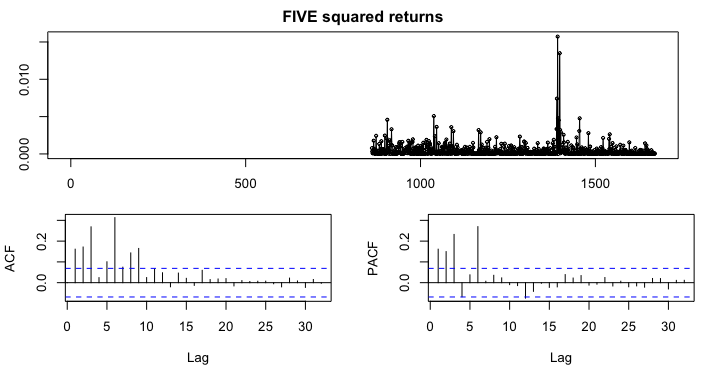
\includegraphics[width=80mm]{five_2.png} \hfill
    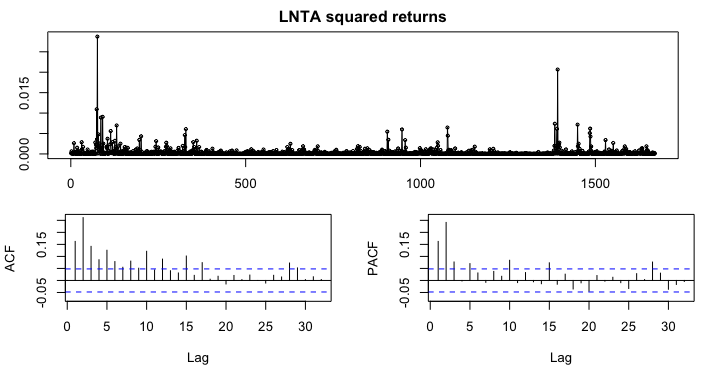
\includegraphics[width=80mm]{lenta_2.png} \hfill
  \end{multicols}
\end{figure}
\begin{figure}[h]
  %\advance\leftskip-1.4cm
    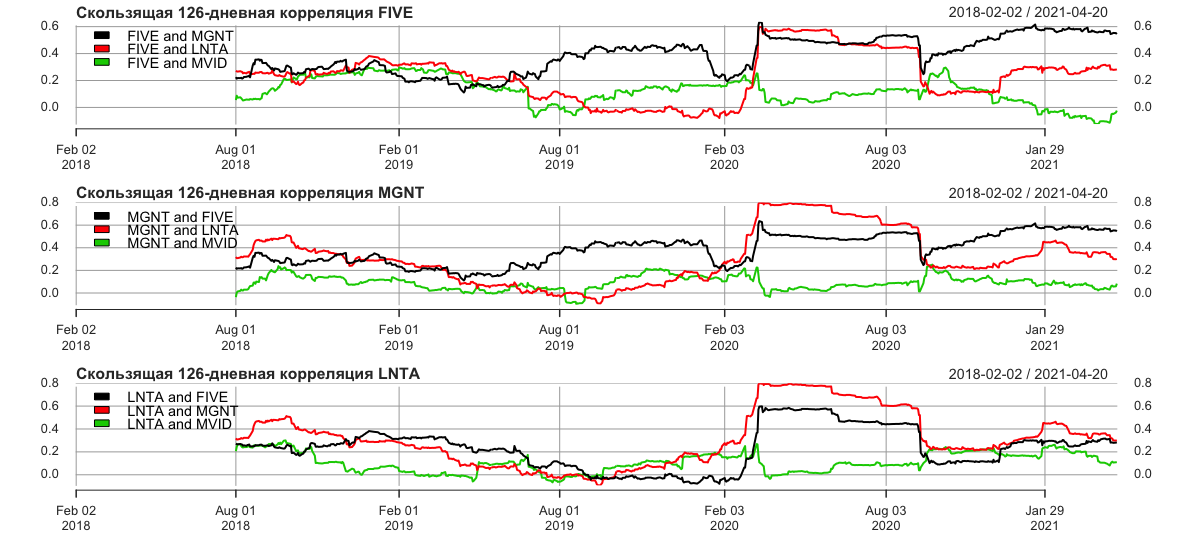
\includegraphics[scale = 0.4]{mult_corr.png}
    \caption{Выборочные корреляции}
    \label{fig:rollcorr2}
\end{figure}

\fcolorbox{green}{lgreen}{Посмотреть чего не хватает}

\end{document} % Конец текста.
